\section{Introduction}

\begin{figure}
    \centering
    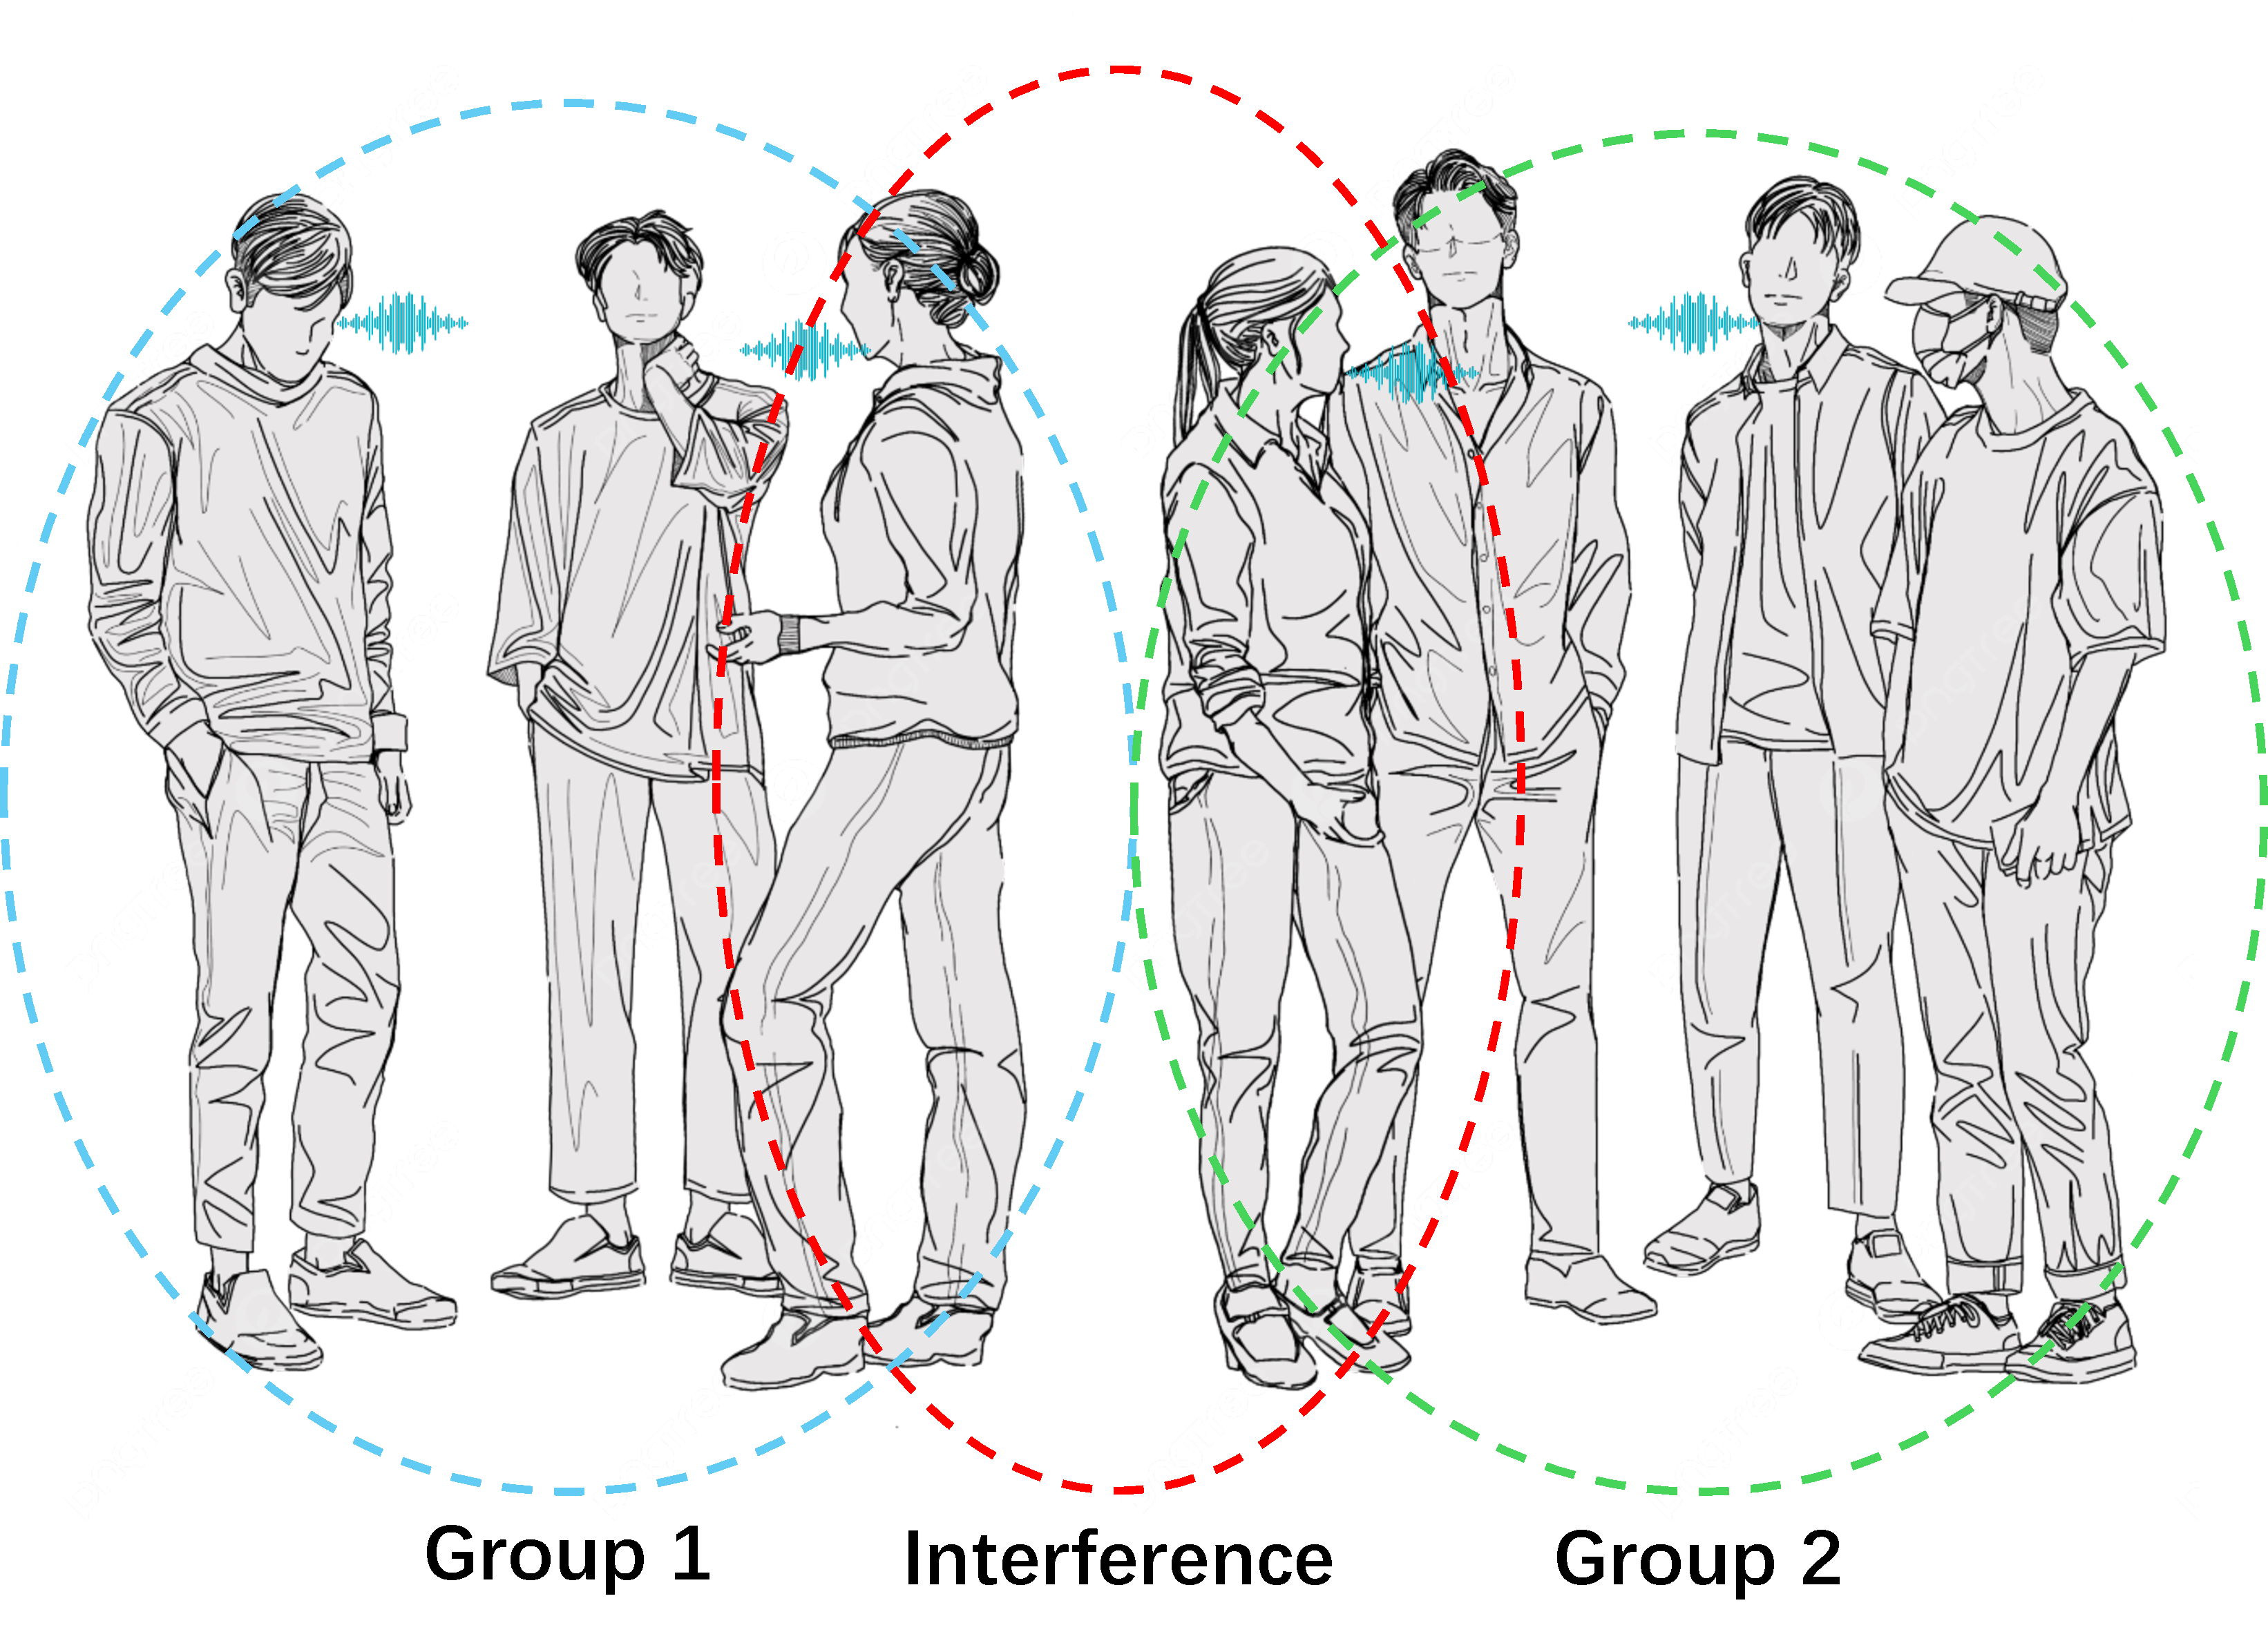
\includegraphics[width=0.6\linewidth]{chapters/cohear/figs/illustration.pdf}
    \vspace{-1em}
    \caption{CoHear uses natural conversational interaction to discover conversation partners and enhance speech within the same conversation group.}
    \label{fig:illustration}
    \vspace{-1em}
\end{figure}

Smart earphones have become a widely deployed wearable platform, with approximately 455 million units shipped globally in 2024 and 11.2\% year-on-year growth~\cite{patentlyapple2025audio}.
Beyond music playback, recent earphone systems support speech enhancement~\cite{chatterjee2022clearbuds, he2023towards, duan2024earse}, speech anti-tampering~\cite{duan2024f2key, hearid}, fine-grained activity recognition~\cite{lyu2024earda}, and spatial audio through IMU-based head tracking~\cite{han2023headmon, han2023headsense, lyu2024earda}. These capabilities make earphones suitable for conversation sensing because they capture both verbal signals and non-verbal cues such as head orientation.

Conversation is an interactive form of communication between two or more people and plays a crucial role in socialization. As illustrated in Fig.~\ref{fig:illustration}, people naturally form separate conversation groups, and ideally, each person wants to focus solely on the members of their own group, regardless of distance or competing voices. The ``cocktail party effect'' \cite{pollack1957cocktail} refers to the human ability to selectively concentrate on a particular voice in noisy environments. However, this perceptual mechanism has limitations. Many individuals experience what is known as ``cocktail party deafness,'' which hinders their ability to follow conversations in crowded settings due to hearing impairments, cognitive overload, or overwhelming background noise \cite{pryse2009companion, cherry1953some}. As a result, clear communication in environments such as conferences, networking events, or guided tours becomes increasingly challenging.


Earphones can therefore serve as assistive tools for conversation listening. However, existing speech enhancement methods do not fully model conversational context. Some methods enhance hearing based on sound categories~\cite{veluri2023semantic}, speaker recognition~\cite{veluri2024look}, or listener distance~\cite{chen2024hearable}, but these cues do not always capture the dynamics of natural conversation. SoundBubble~\cite{chen2024hearable}, for example, assumes a defined spatial region, while real conversations may form across irregular distances and orientations. The method in~\cite{chen2024target} extracts conversations based on turn-taking dynamics and previously recorded audio, but its reliance on turn-taking events introduces delay and limits real-time use.


To address these limitations, CoHear uses multi-device collaboration for conversation enhancement. In contrast to earphone systems that focus on single-device processing~\cite{dong2024rehearsse, he2023towards, duan2024earse}, CoHear treats conversation as a multi-user activity. It connects individual earphones into a lightweight network and combines wearable sensing with distributed acoustic observations.


The CoHear earphone network departs from the conventional assumptions of wireless acoustic sensor networks in two ways~\cite{gburrek2021geometry}. Traditionally, such networks assume that (1) sound sources appear randomly and independently of sensor node placement, and (2) the sensor nodes themselves remain static. In contrast, the conversation-driven setting has a different structure: the sound sources, i.e., human speakers, are co-located with mobile sensor nodes (earphones), and these nodes dynamically organize themselves into conversation groups, as illustrated in Fig.~\ref{fig:illustration}.
Consequently, the conversation network is triggered and constructed by interactions among users, which can be modeled through verbal or non-verbal features. Verbal features such as turn-taking are delayed and sensitive to interference, so CoHear primarily uses non-verbal features such as head orientation to infer conversation groups.

To establish the conversation network, CoHear uses multi-channel audio and IMU recordings to detect nearby speakers, estimate their locations, and infer conversations from relative orientations. The enhanced speech can then be rendered through noise-canceling earphones. Implementing this system raises three challenges:
\begin{itemize}
    \item \textbf{Dynamic peer discovery and network formation.} Since conversations occur spontaneously and participants are mobile, the system must continuously identify nearby speakers, localize their positions, and group devices into socially coherent clusters without any fixed infrastructure.

    \item \textbf{Topology estimation and coordination.}
    The estimation and observations of a single user may be insufficient to identify conversation participants. Therefore, aggregating the noisy, distributed observations from heterogeneous devices is necessary for establishing a global coordinate system to locate conversations.

    \item \textbf{Conversation enhancement.}
    Even a well-established conversation network may not be directly useful to users without additional processing. The earphone platform enables targeted extraction of conversation-level speech, but the system must select and use conversation conditions, such as speaker embeddings, from the network under latency and bandwidth constraints.
\end{itemize}



To address these challenges, CoHear makes three contributions:
\begin{enumerate}
    \item \textbf{A conversation network for earphones.}
    CoHear designs a conversation network that uses earphone sensing to model conversation groups without fixed infrastructure. The network includes two components:
    (i) a node discovery module that detects nearby speakers along with their locations and speaker embeddings, as described in Sec. \ref{sec:cohear_acoustic}. This task is divided into two parts: sound source localization and speaker embedding extraction. A joint identity extraction model is used to integrate these two elements.
    (ii) a geometric calibration pipeline that estimates the global network topology using the output from node discovery, as detailed in Sec. \ref{sec:cohear_geometric}. This pipeline matches sound sources identified across different devices, calculates the distances between them, and uses this information for geometric calibration.

    \item \textbf{Bandwidth-aware target conversation enhancement.}
    Based on the network structure, CoHear develops a conversation enhancement module for low latency and bandwidth efficiency. This module uses peer-relayed audio as conditioning signals and remains effective under network delays, packet loss, and compression artifacts. An adaptive model uses both time-invariant and time-varying conditioning features, while an audio control module manages feature selection and bandwidth usage.

    \item \textbf{A practical implementation with real-world validation.}
    CoHear is implemented on earphones equipped with microphones and IMUs. Real-world experiments, simulations, and user studies show over 90\% accuracy in conversation group formation, up to 8.8 dB SNR improvement over representative baselines, and real-time performance (RTF > 1) on mobile devices. An adaptive bandwidth controller further improves performance under constrained conditions.
\end{enumerate}
